\subsubsection{Interfaces de Usuario}\label{Interfaces de Usuario}

A continuación se muestra la pantalla principal que será visible siempre que se inicie la aplicación, bajo la barra de navegación encontraremos una barra de selección de sensor del sistema del cual visualizaremos la gráfica con las muestras tomadas durante el transcurso del día, por defecto mostrará los del primer o único sensor. En la parte inferior vamos a poder observar la mejor marca de producción del día en Kw/Hr, y debajo de esta el estado de generación actual, es decir, el valor sensado en ese mismo instante de tiempo en el que mantenemos abierta la aplicación, el cual se actualizará cada segundo. En la parte superior izquierda cuenta con una barra de navegación la cual nos permite acceder a otros componentes de la aplicación.  

\begin{figure}[H]
	\centering
	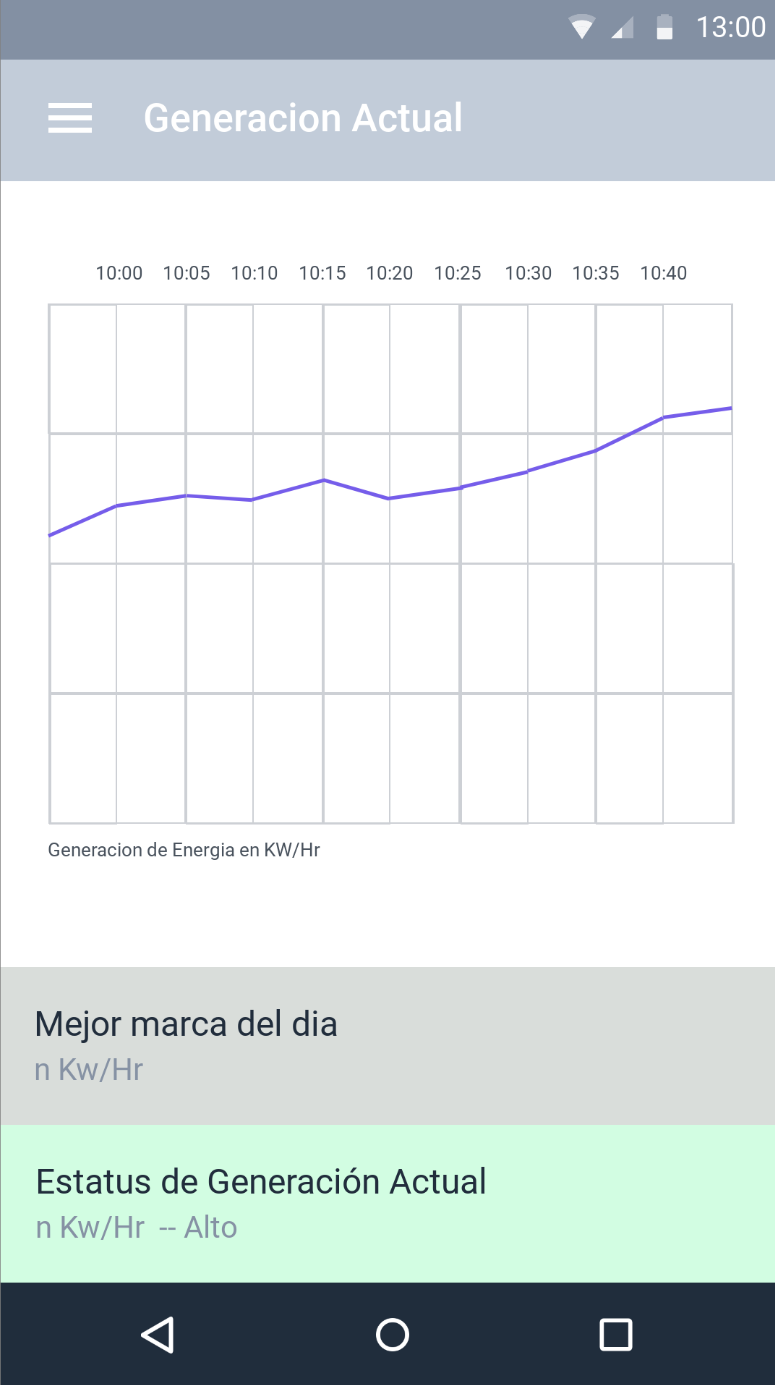
\includegraphics[scale=0.70]{Capitulo4/software/submodulos/images/monitoreo.png}
	\caption{Interfaz de usuario IU1.1-Ver Generación En Tiempo Real}
	\label{fig:monitoreo}
\end{figure}

\begin{figure}[H]
	\centering
	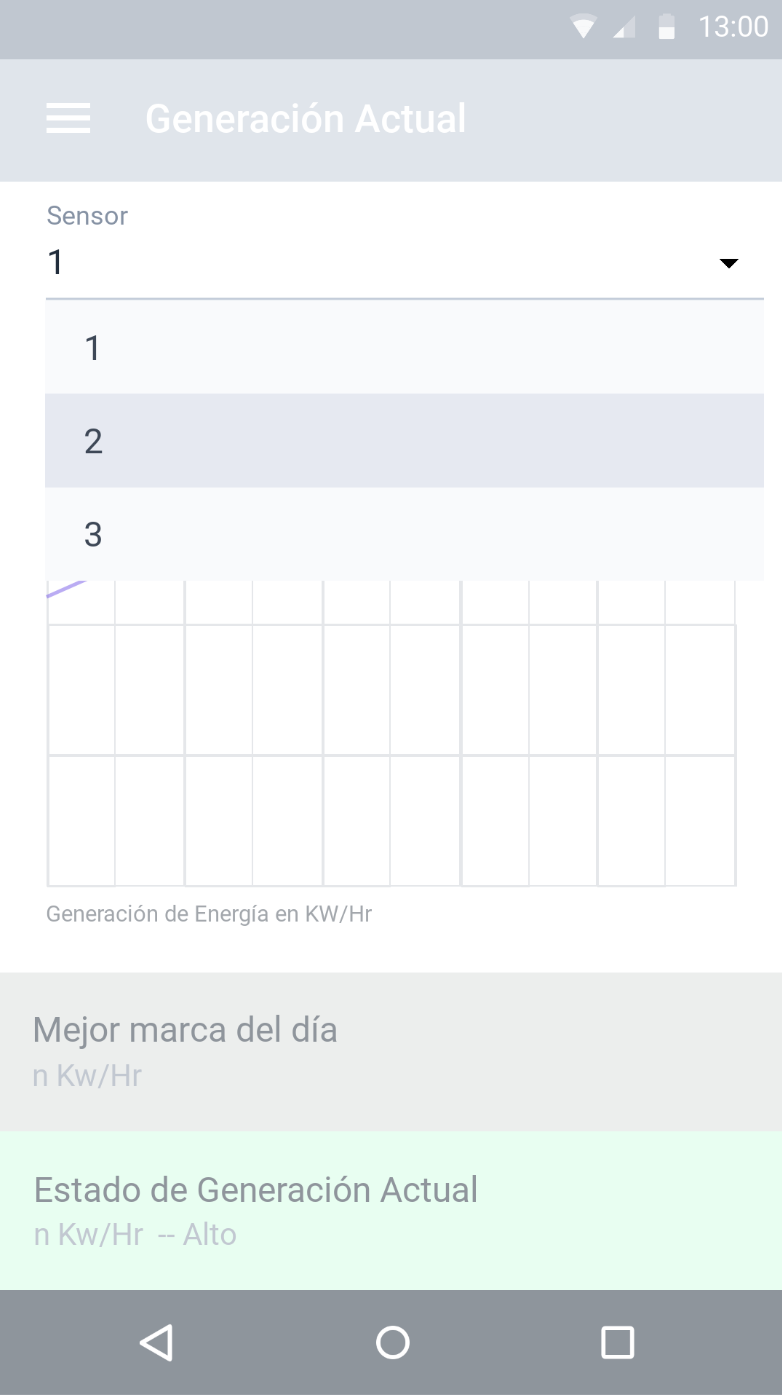
\includegraphics[scale=0.70]{Capitulo4/software/submodulos/images/monitoreo_sel.png}
	\caption{Interfaz de usuario IU1.2-Ejemplo de opciones de selección de sensor}
	\label{fig:monitoreo}
\end{figure}

La pantalla mostrada a continuación contiene las 4 posibles opciones que tiene la barra de navegación de la pantalla principal \ref{fig:monitoreo}, cada uno de los 4 botones nos redirige a un componente de la aplicación.

\begin{figure}[H]
	\centering
	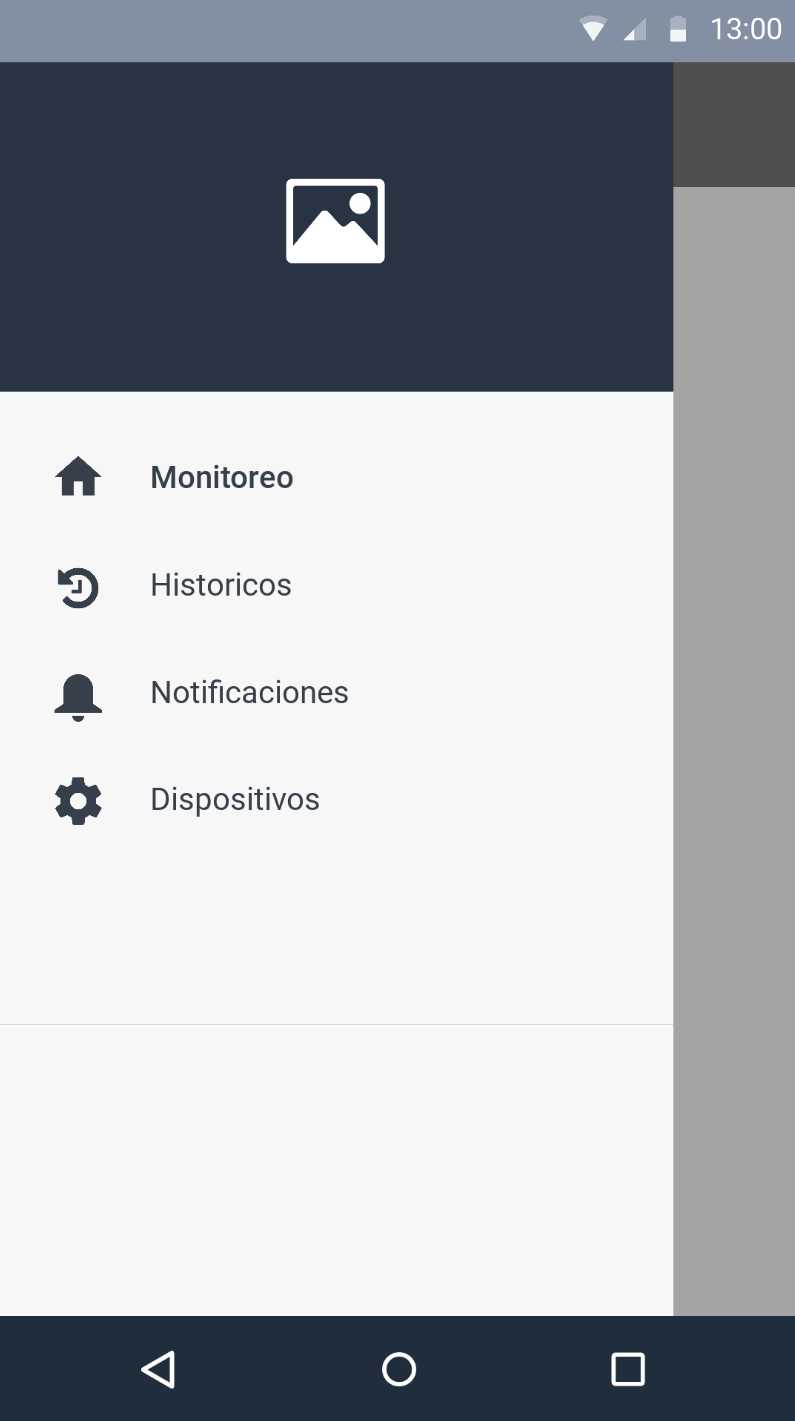
\includegraphics[scale=0.70]{Capitulo4/software/submodulos/images/navegacion.png}
	\caption{Interfaz de usuario IU5-Barra de Navegación}
	\label{fig:Barra de navegacion}
\end{figure}

En la siguiente pantalla podemos observar la pantalla de históricos (opción disponible en la barra de navegación de la pantalla \ref{fig:Barra de navegacion}) , la cual por defecto siempre que sea accedida mostrará la gráfica de generación semanal y con el primer o único sensor. La pantalla posee dos barras de selección, una en donde podremos seleccionar los 3 diferentes periodos a graficar, es decir, semanal, mensual y bimestral, y la segunda donde podremos seleccionar de que sensor del sistema nos mostrará la información histórica. 

\begin{figure}[H]
	\centering
	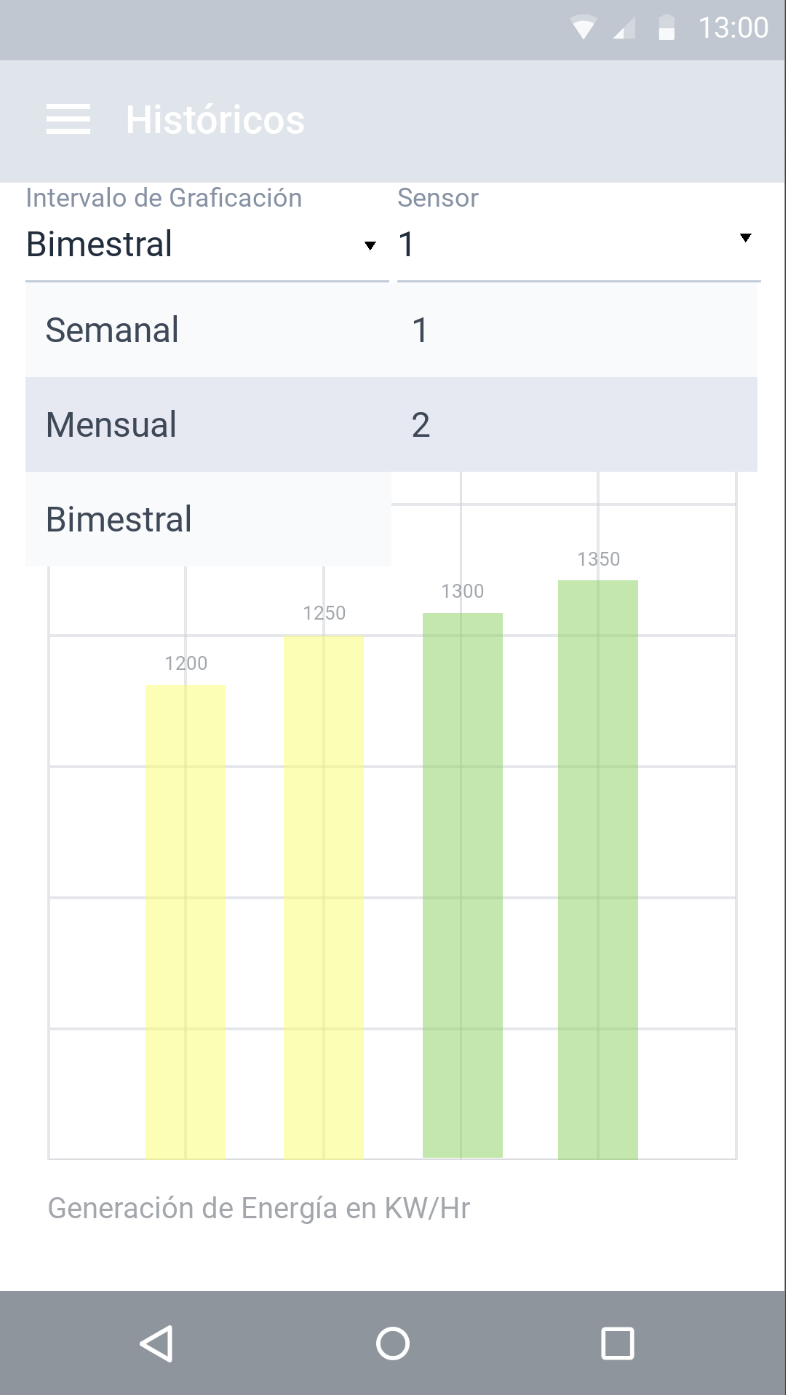
\includegraphics[scale=0.70]{Capitulo4/software/submodulos/images/opciones_hist.png}
	\caption{Interfaz de usuario IU2.4-Opciones de Intervalo}
	\label{fig:Opciones de Intervalo}
\end{figure}

La siguientes 3 pantallas muestran la producción de energía que es sensada en distintos periodos mediante una gráfica de barras, la figura \ref{fig:Historial Semanal} grafica de acuerdo al periodo semanal, la figura \ref{fig:Historial Mensual} de acuerdo al periodo mensual y por último, la figura \ref{fig:Historial Bimestral} de acuerdo al periodo bimestral, de esta manera podemos tener un mejor control sobre la energía que el sistema está produciendo. 

\begin{figure}[H]
	\centering
	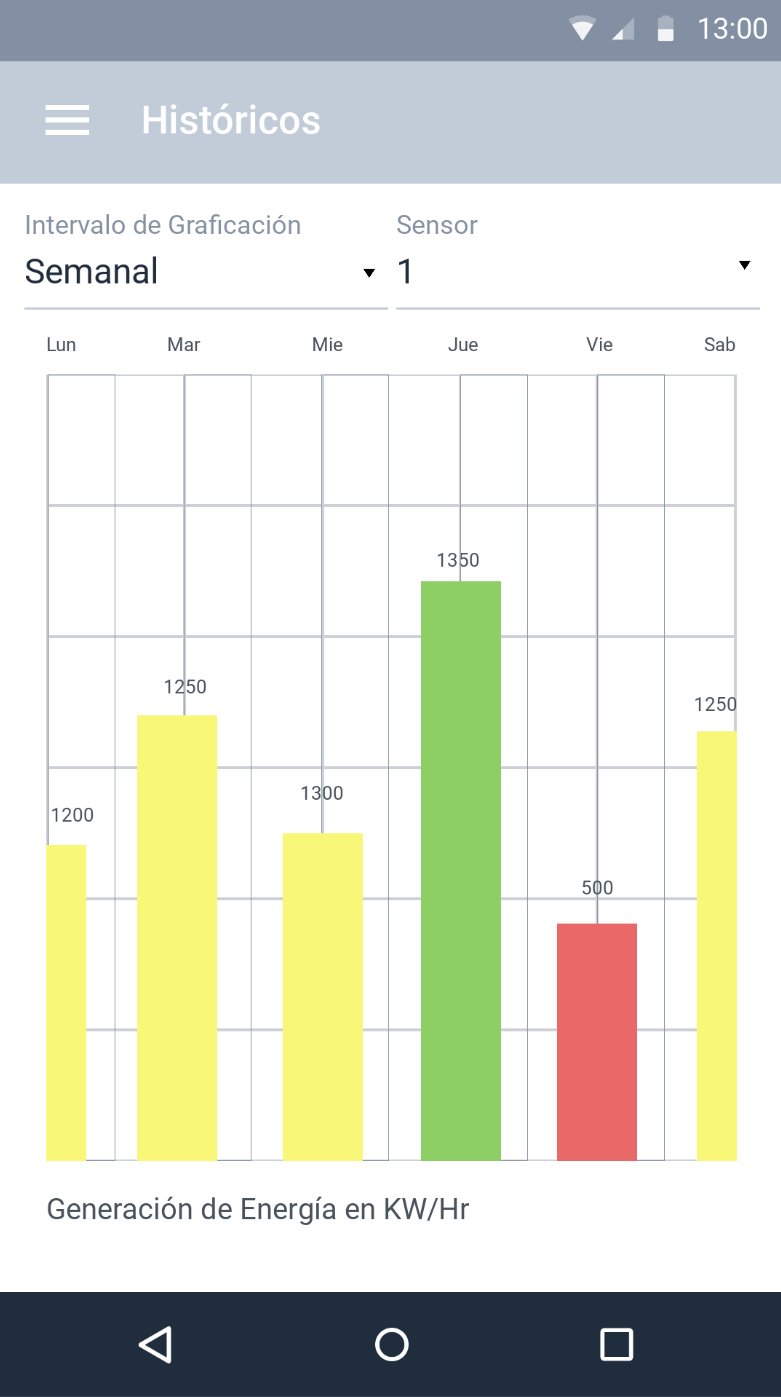
\includegraphics[scale=0.70]{Capitulo4/software/submodulos/images/semanal.png}
	\caption{Interfaz de usuario IU2.1-Historial Semanal}
	\label{fig:Historial Semanal}
\end{figure}

\begin{figure}[H]
	\centering
	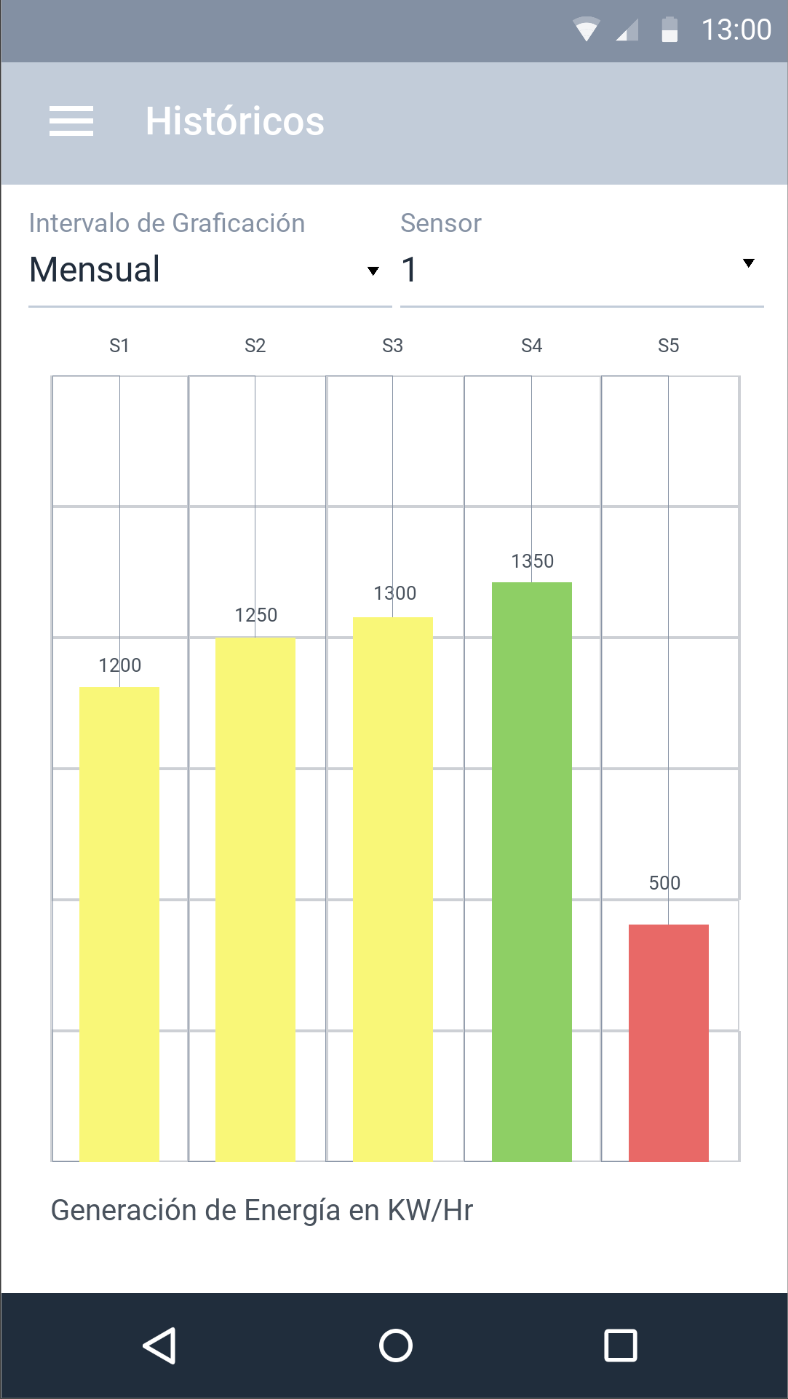
\includegraphics[scale=0.70]{Capitulo4/software/submodulos/images/mensual.png}
	\caption{Interfaz de usuario IU2.2-Historial Mensual}
	\label{fig:Historial Mensual}
\end{figure}

\begin{figure}[H]
	\centering
	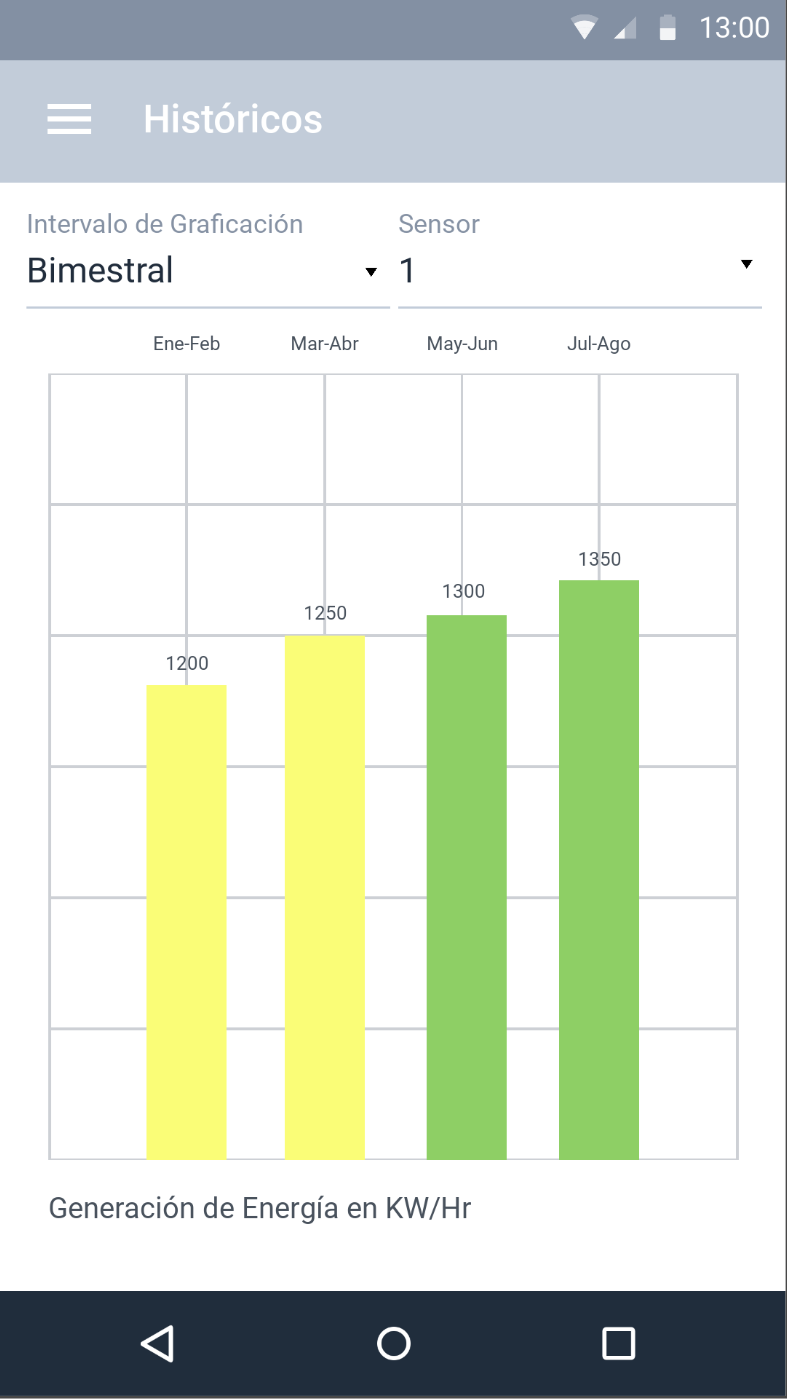
\includegraphics[scale=0.70]{Capitulo4/software/submodulos/images/bimestral.png}
	\caption{Interfaz de usuario IU2.3-Historial Bimestral}
	\label{fig:Historial Bimestral}
\end{figure}

La pantalla siguiente (opción disponible en la barra de navegación de la pantalla \ref{fig:Barra de navegacion}) indica en el primer campo el dispositivo actual con el que se tiene conexión, es decir, el servidor que es el encargado de dar respuesta a las peticiones hechas por la aplicación móvil, por otro lado, en el campo inferior se muestran los dispositivos disponibles con los que se puede hacer conexión, pero también se le es permitido al usuario ingresar la IP de un nuevo dispositivo con el que se desee realizar una conexión.

\begin{figure}[H]
	\centering
	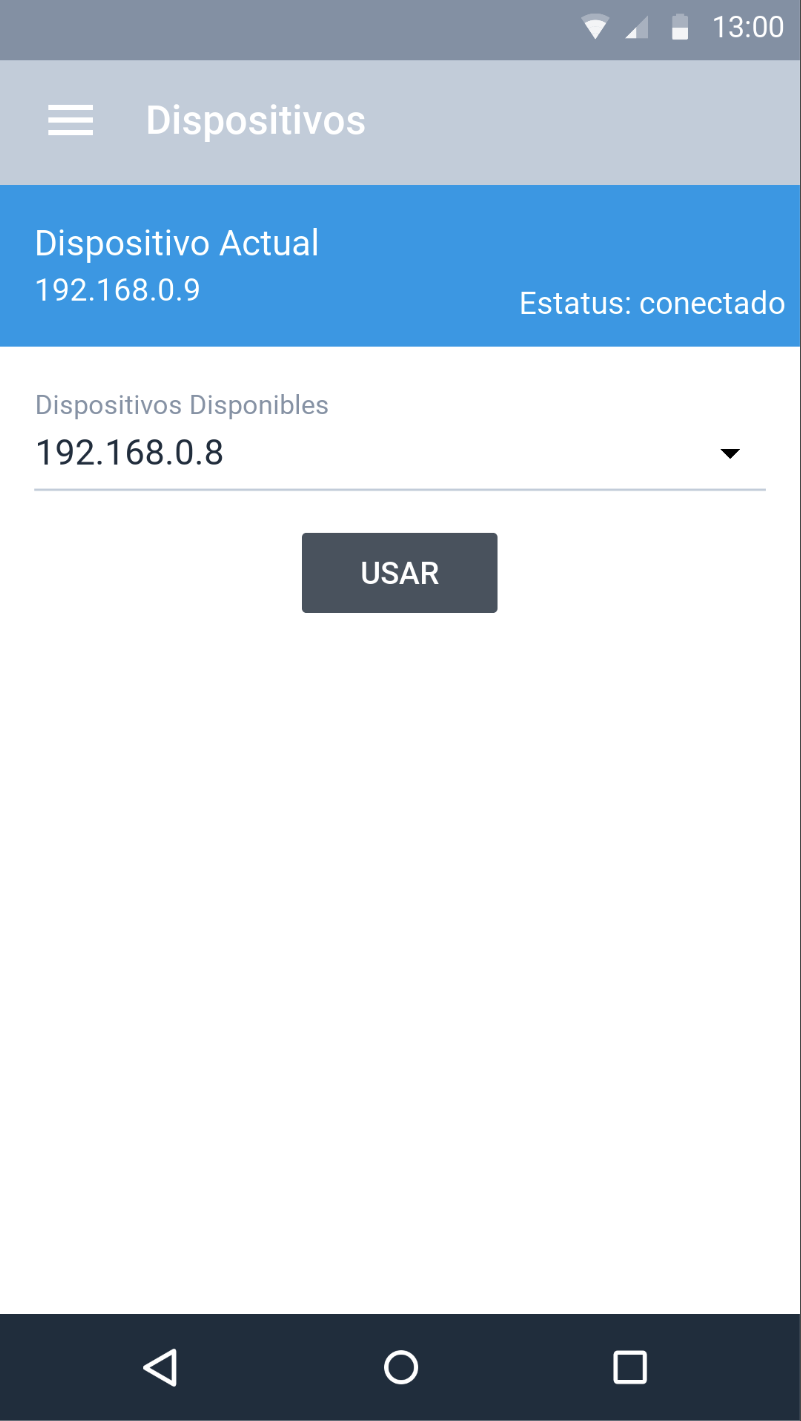
\includegraphics[scale=0.70]{Capitulo4/software/submodulos/images/dispositivos.png}
	\caption{Interfaz de usuario IU3.1-Emparejamiento de Dispositivos}
k	\label{fig:Emparejamiento Dispositivo}
\end{figure}

Como se explica en la pantalla anterior, si damos clic en los dispositivos disponibles se despliega una lista con los dispositivos con los que se puede realizar una conexión, esto es visible en la pantalla mostrada a continuación.

\begin{figure}[H]
	\centering
	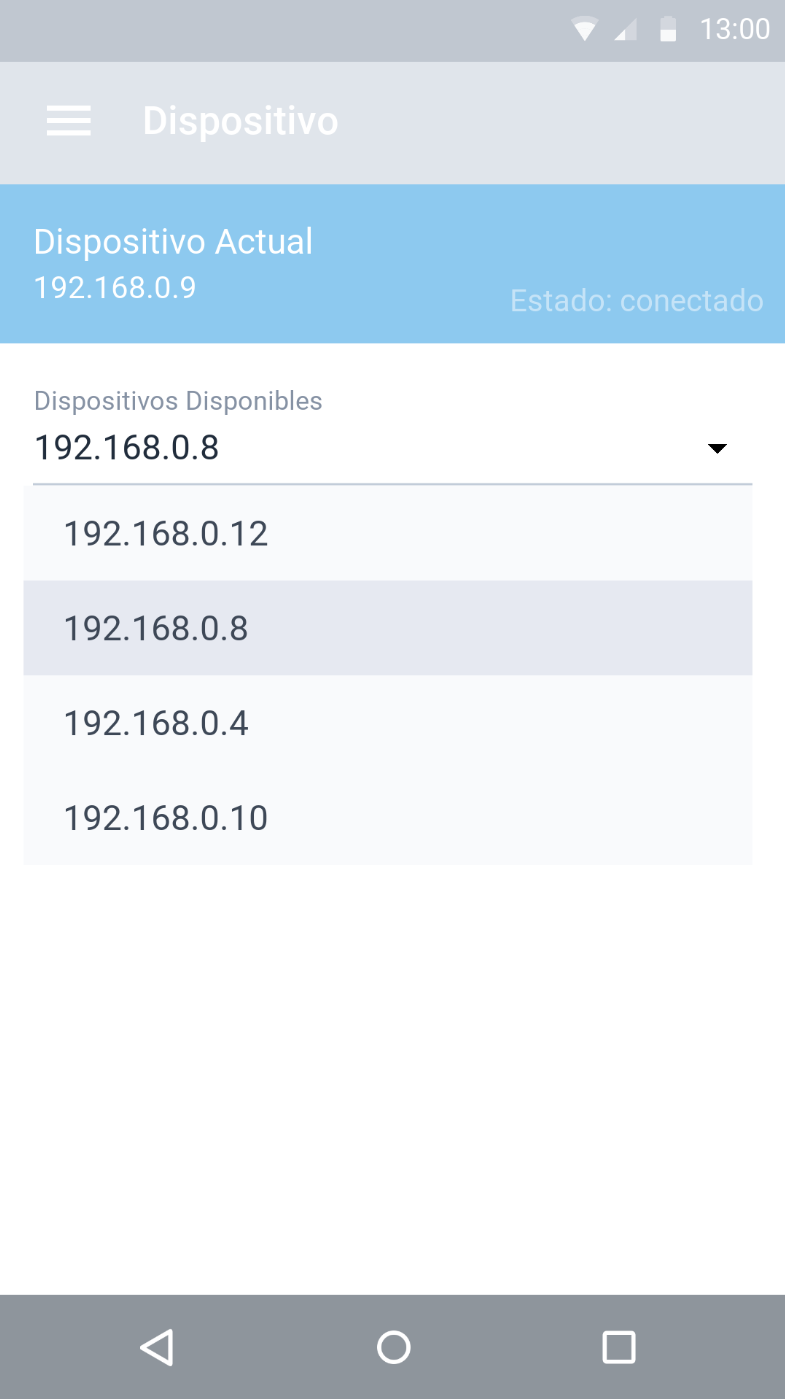
\includegraphics[scale=0.70]{Capitulo4/software/submodulos/images/opciones_disp.png}
	\caption{Interfaz de usuario IU3.2-Selección de Dispositivo}
	\label{fig:Seleccion de Disposotivo}
\end{figure}

La pantalla siguiente (opción disponible en la barra de navegación de la pantalla \ref{fig:Barra de navegacion}) muestra la lista de notificaciones almacenadas que han ido surgiendo en el transcurso en el que ha sido usada la aplicación.

\begin{figure}[H]
	\centering
	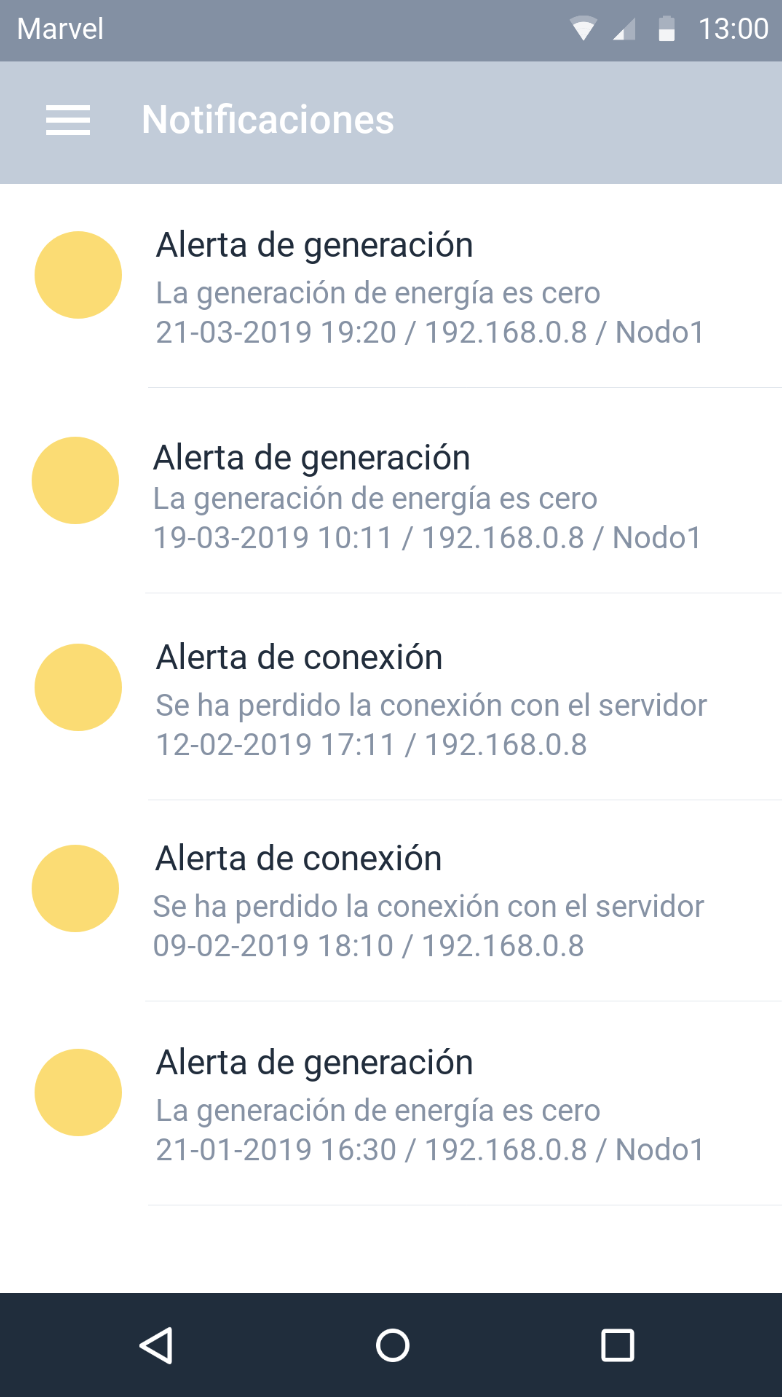
\includegraphics[scale=0.70]{Capitulo4/software/submodulos/images/notificaciones.png}
	\caption{Interfaz de usuario IU4-Lista de Notificaciones}
	\label{fig:Lista de Notificaciones}
\end{figure}


\subsubsection{Pantallas emergentes}\label{Pantallas Emergentes}

Las pantallas emergentes son pequeños mensajes para notificar al usuario sobre algo en específico, la pantalla emergente mostrada a continuación ayuda a alertar al usuario sobre un problema de conexión con el servidor embebido.

\begin{figure}[H]
	\centering
	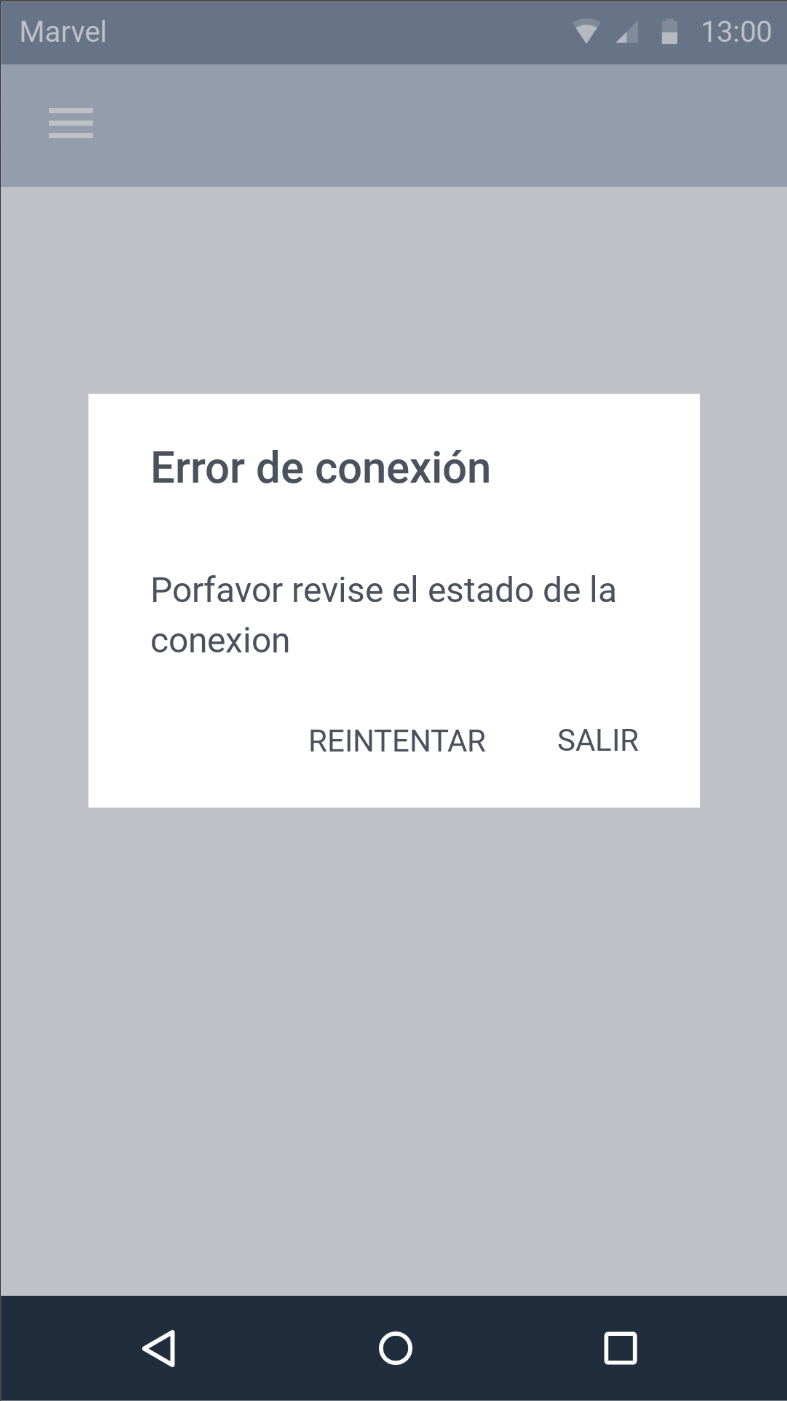
\includegraphics[scale=0.70]{Capitulo4/software/submodulos/images/error_con.png}
	\caption{Pantalla emergente PE1-Error de Conexión}
	\label{fig:Error de Conexion}
\end{figure}

La pantalla emergente mostrada a continuación alerta sobre un error en el servidor y como recomendaciones pide revisar el servidor o el sistema fotovoltaico.

\begin{figure}[H]
	\centering
	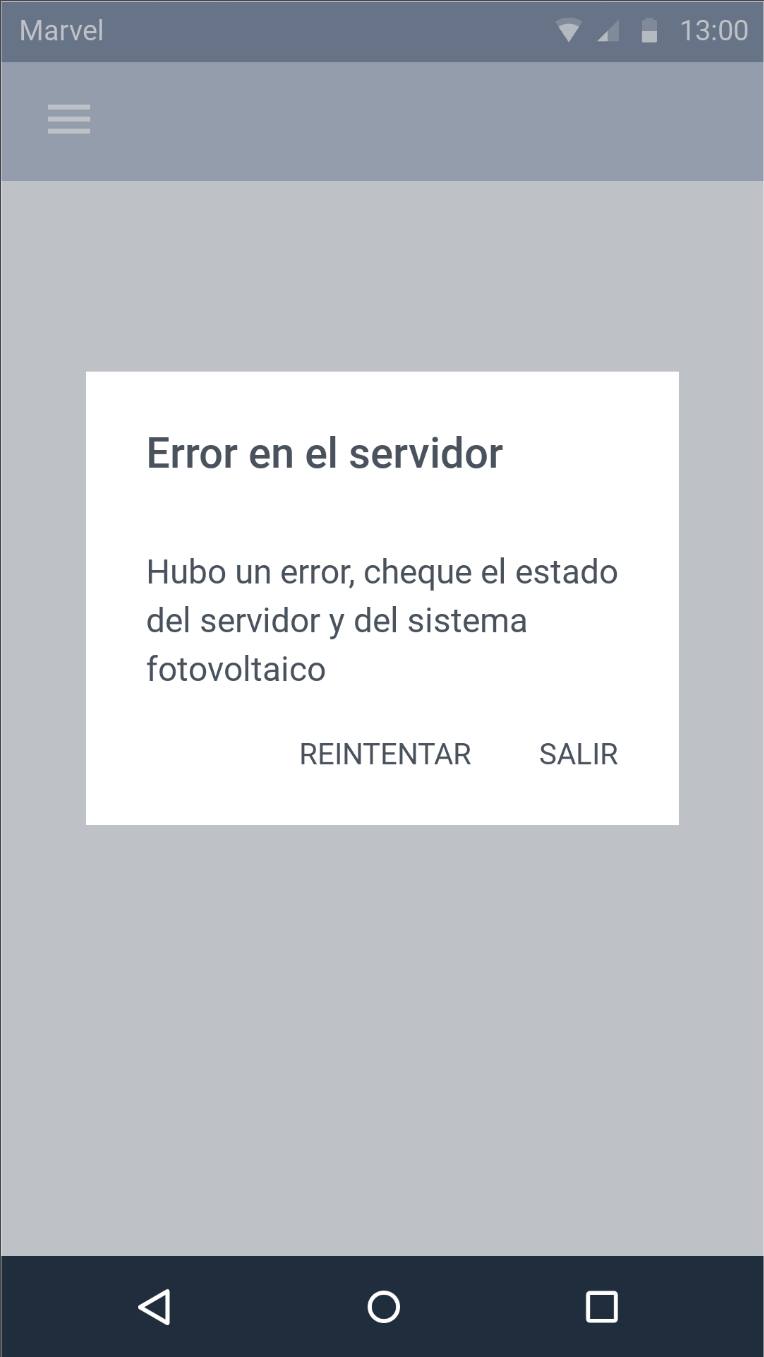
\includegraphics[scale=0.70]{Capitulo4/software/submodulos/images/error_server.png}
	\caption{Pantalla emergente PE2-Error en el Servidor}
	\label{fig:Error en el Servidor}
\end{figure}

Esta pantalla emergente muestra un mensaje de éxito en la conexión, esto para avisar al usuario que el emparejamiento con el sistema embebido se ha realizado de manera correcta.

\begin{figure}[H]
	\centering
	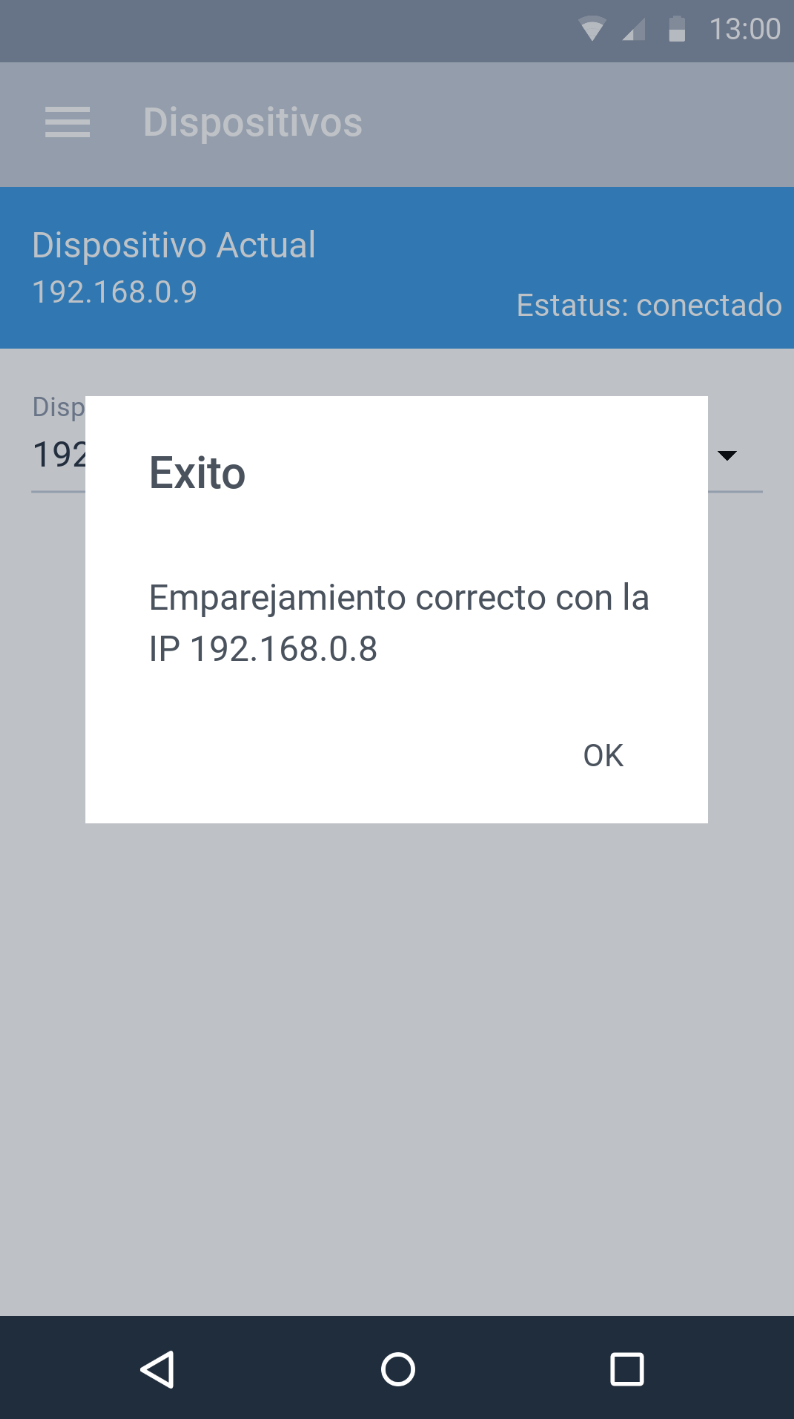
\includegraphics[scale=0.70]{Capitulo4/software/submodulos/images/exito_disp.png}
	\caption{Pantalla emergente PE3-Éxito de Emparejamiento con Dispositivo}
	\label{fig:Exito Emparejamiento}
\end{figure}

Por el lado contrario, la pantalla emergente que se muestra a continuación alerta sobre un error al momento de establecer una conexión.

\begin{figure}[H]
	\centering
	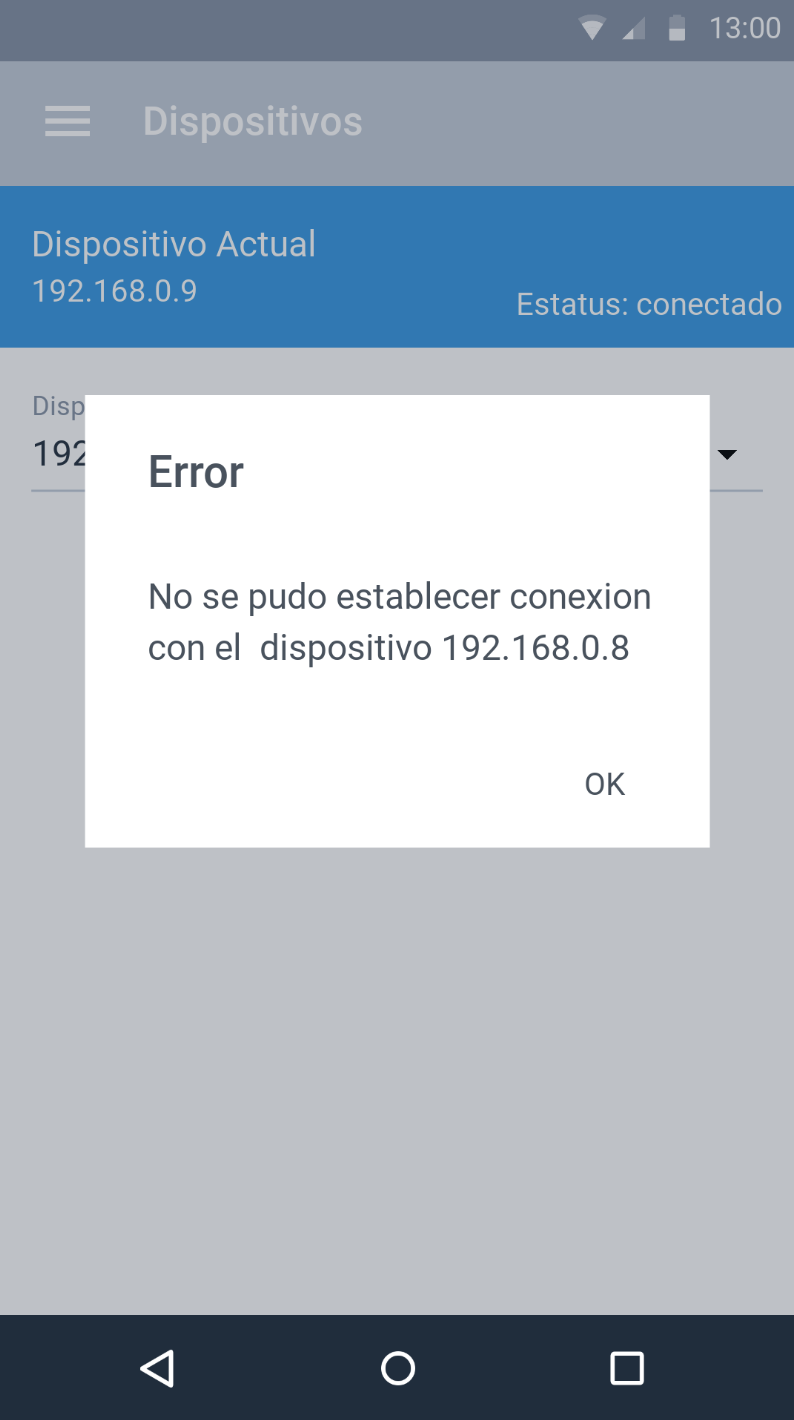
\includegraphics[scale=0.70]{Capitulo4/software/submodulos/images/error_disp.png}
	\caption{Pantalla emergente PE4-Error de Emparejamiento con Dispositivo}
	\label{fig:Error Emparejamiento}
\end{figure}

\subsubsection{Notificaciones}\label{Notificaciones}

Las notificaciones como tal no son pantallas emergentes, sin embargo su funcionalidad es similar, notificar al usuario sobre algo en específico, en este caso de una anomalía, a continuación se muestran únicamente 3 anomalías que podrá notificar la aplicación, La pantalla \ref{fig:Alerta Conexion} muestra la notificación por problemas de conexión con el servidor, la pantalla \ref{fig:Alerta Generacion} por interrupción de generación de energía y la pantalla \ref{fig:Alerta Servidor} por problemas con el servidor embebido. 

\begin{figure}[H]
	\centering
	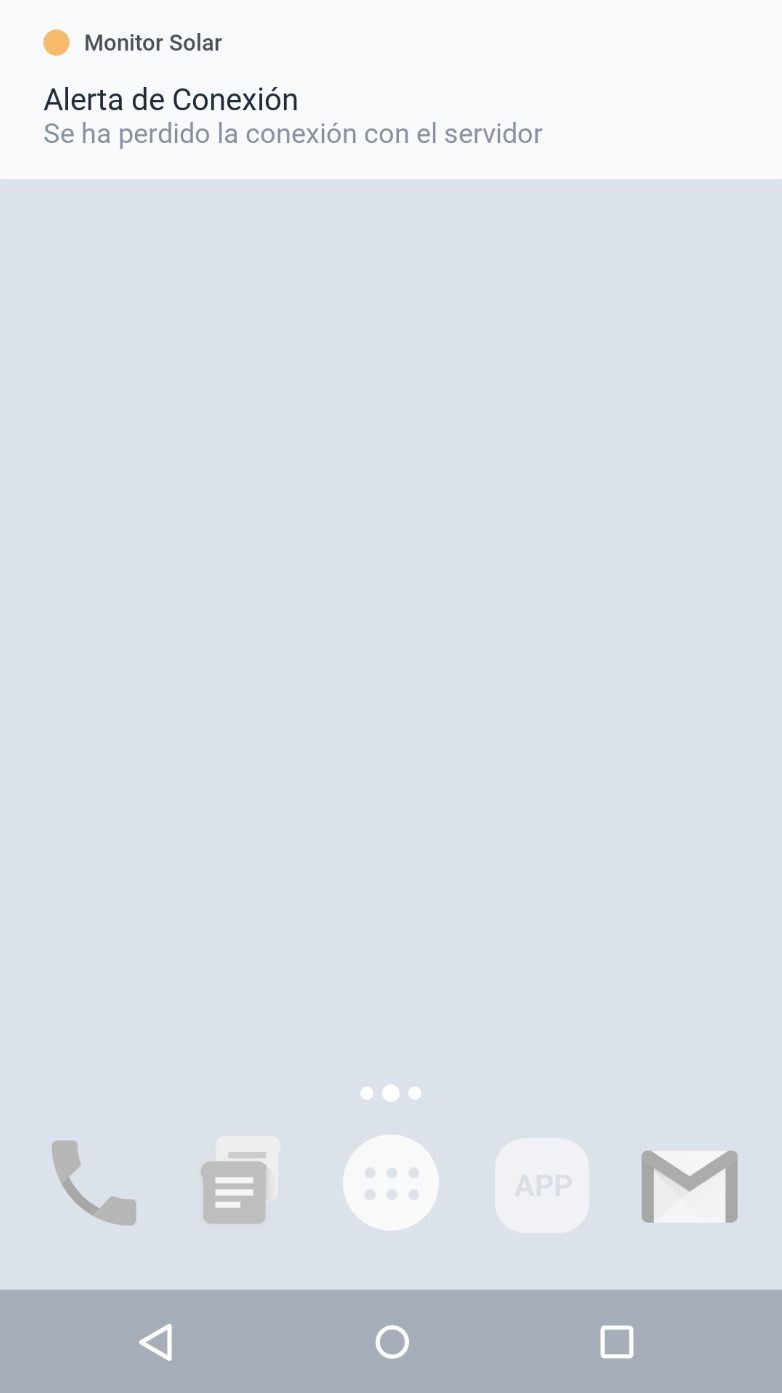
\includegraphics[scale=0.70]{Capitulo4/software/submodulos/images/notif_con.png}
	\caption{Notificación N1-Alerta de Conexión}
	\label{fig:Alerta Conexion}
\end{figure}

\begin{figure}[H]
	\centering
	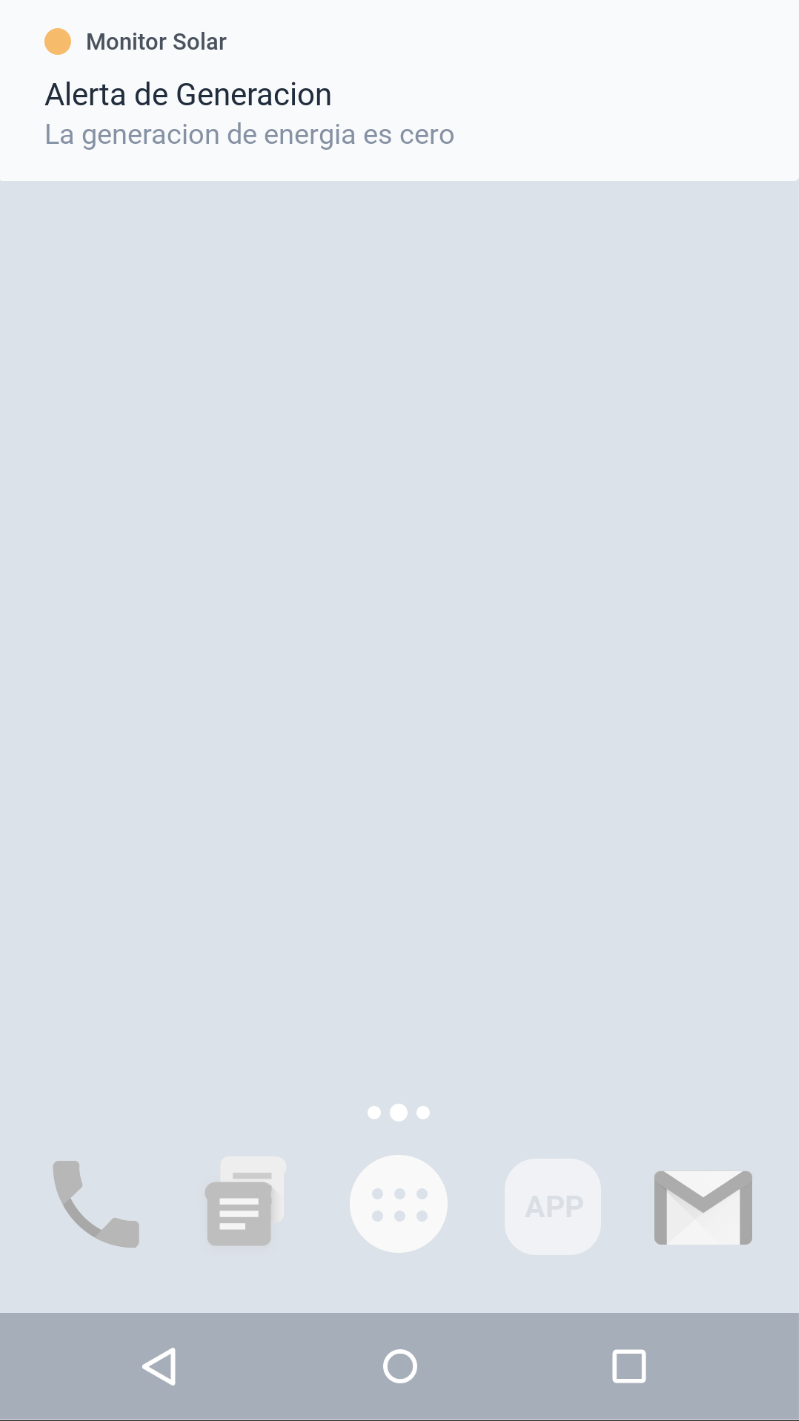
\includegraphics[scale=0.70]{Capitulo4/software/submodulos/images/notif_gen.png}
	\caption{Notificación N2-Alerta de Generación}
	\label{fig:Alerta Generacion}
\end{figure}

\begin{figure}[H]
	\centering
	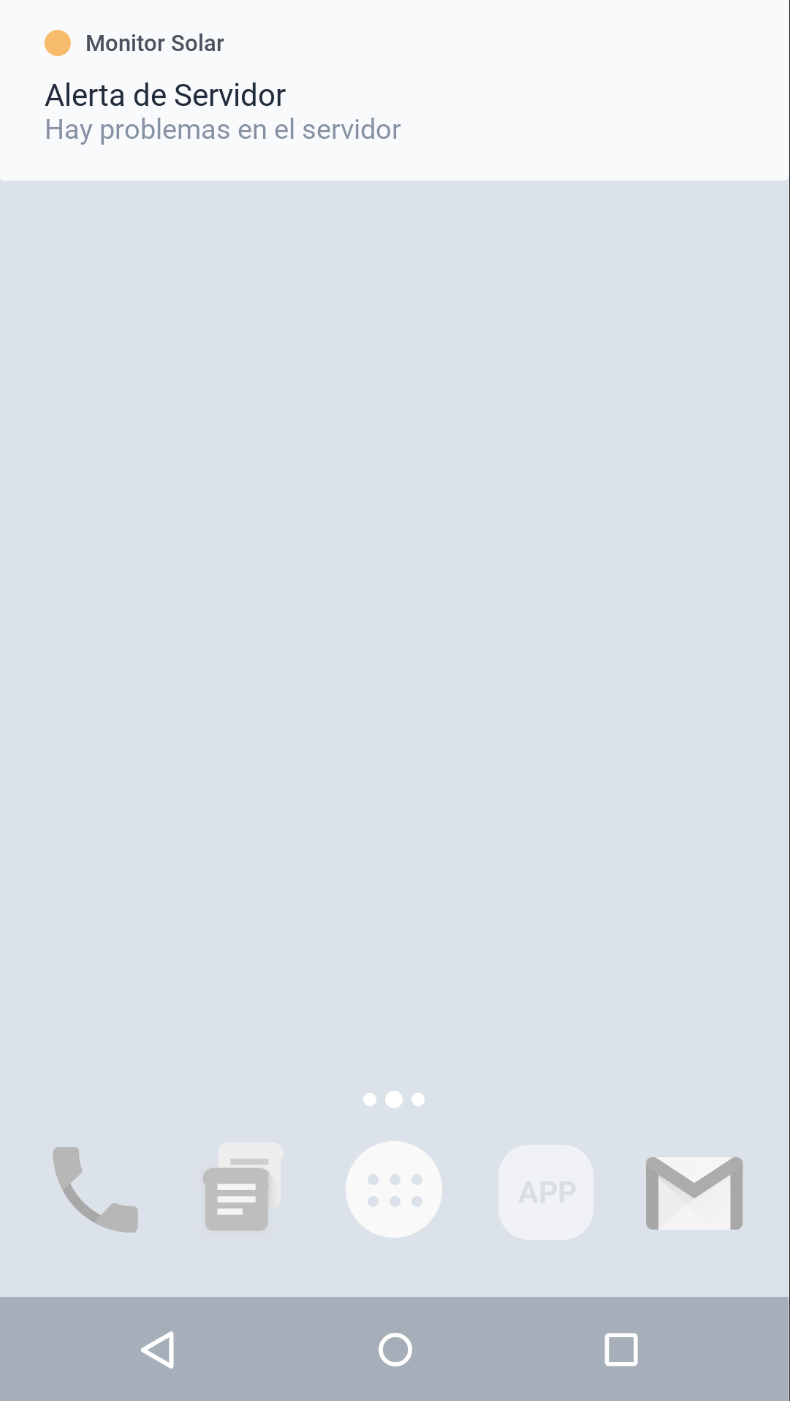
\includegraphics[scale=0.70]{Capitulo4/software/submodulos/images/notif_server.png}
	\caption{Notificación N2-Alerta de Servidor}
	\label{fig:Alerta Servidor}
\end{figure}